\documentclass[12pt]{article}
\usepackage[utf8]{inputenc}
\usepackage{polski}
\usepackage[a4paper, left=2.0cm, right=2.0cm, top=2.0cm, bottom=2.0cm]{geometry}
\usepackage{graphicx}
\usepackage{multicol}
\usepackage{hyperref}


\title{PIISW, W08, IO, 2020/2021, semestr letni\\Lista zadań nr 3: Tworzenie i testowanie backendu: serwisy RESTowe}
\author{Maciej Małecki\\ \small maciej.malecki@pwr.edu.pl}

\begin{document}
    \maketitle

    \section*{Zasady Pracy}
    \begin{itemize}
        \item Rozwiązania zadań muszą być umieszczone w~prywatnym repozytorium na portalu \texttt{git\-hub.com}.
        \item Prowadzący musi mieć uprawnienia do odczytu i~zapisu dla tego repozytorium.
        \item Zadanie~\ref{exc:spring_rest} jest obowiązkowe -- w~razie jego braku dalsza część listy nie będzie sprawdzana.
    \end{itemize}

    \section*{Wprowadzenie}
        W~zadaniu \ref{exc:spring_rest} należy zaimplementować uproszczoną wersję reverse-proxy.
        Reverse-proxy nie ma żadnej logiki biznesowej i~służy jedynie jako pośrednik odbierający żądania i~przekazujący je dalej.
        Reverse-proxy ukrywa architekturę systemów po stronie odbiorcy przed nadawcą, on (nadawca) niezależnie od rodzaju żądania cały czas rozmawia z~jednym systemem.

    \section*{Oceny}
    \begin{tabular}{|l|c|c|c|c|c|c|}
        \hline
        Punkty: & $<7$ & $7-8$ & $9-10$ & $11-12$ & $13-14$ & 15\\
        \hline
        Ocena: & $2,0$ & $3,0$ & $3,5$ & $4,0$ & $4,5$ & $5,0$\\
        \hline
    \end{tabular}

    \section*{Zadania}
    \begin{enumerate}
        \item\label{exc:spring_rest}
            (4 pkt) Reverse-Proxy - zadanie podstawowe.\\
            Zaimplementuj szary element z~rysunku~\ref{fig:lista_3_proxy}, posiadający interfejsy RESTowe: wejściowy i~wyjściowy.
            \begin{itemize}
                \item Interfejs wejściowy przyjmuje żądanie od nadawcy i~w~zależnosci od jego typu przekazuje do odpowiedniego adresata (system 1-3). Gdy adresat przetworzy żądanie, jego odpowiedź jest zwracana do nadawcy.
                \item Ponieważ systemy zewnętrzne nie istnieją, należy je "zamokować" z~użyciem dowolnego narzędzia (wiremock, json-server, \ldots).
                \item Konfiguracja adresów systemów zewnętrznych powinna znaleźć się w~pliku \texttt{applica\-tion.pro\-per\-ties} w~formie np. \texttt{destination.get=localhost:8899}.
            \end{itemize}
            
            \begin{figure}[ht]
                \centering
                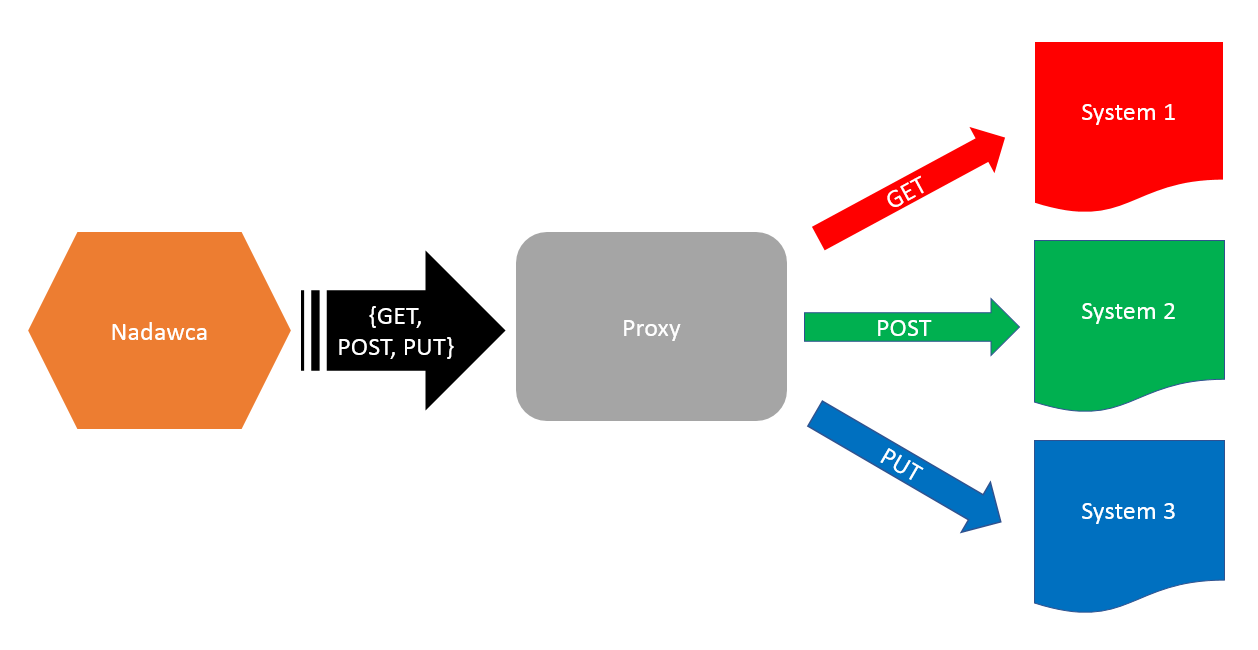
\includegraphics[width=\textwidth]{lista_3_proxy}
                \caption{Diagram obrazujący sposób działania reverse proxy implementowanego w ramach zadania~\ref{exc:spring_rest}.}
                \label{fig:lista_3_proxy}
            \end{figure}

            \textbf{Wskazówka:} Wygeneruj aplikację SpringBoot z~wykorzystaniem Maven oraz z~modułem Web (wykorzystaj w~tym celu \url{https://start.spring.io}) oraz zaznajom się z~\texttt{RestController} i~\texttt{RestTemplate}.

        \item\label{exc:spring_rest_test}
            (3 pkt) Testowanie automatyczne.\\
            Napisz testy automatyczne dla komponentu reverse-proxy stworzonego w~zadaniu~\ref{exc:spring_rest}.
            \begin{itemize}
                \item Dla każdego rodzaju żądania należy napisać co najmniej jeden test automatyczny.
                \item Jeśli rodzaj testu tego wymaga, zależność (czyli obecność systemu będącego na końcu testowanego interfejsu) powinna być uruchamiana przez sam test, a~nie przez użytkownika -- ręcznie.
            \end{itemize}

            \textbf{Wskazówka:} Zaznajom się z~\texttt{TestRestTemplate} oraz np. \texttt{Wiremock} i~jego wsparciem dla testów JUnit.

        \item\label{exc:spring_exception_handling}
            (2 pkt) Obsługa wyjątków.\\
            Reverse-proxy nie interpretuje błędów, jakie mogą wystąpić podczas komunikacji systemami zewnętrznymi. Błędy takie należy przekazywać dalej.
            \begin{itemize}
                \item Do obsługi wyjątków należy użyć \texttt{ControllerAdvice}.
                \item W~zależnosci od implementacji testy automatyczne powinny być rozszerzone o~przypadki sprawdzające sytuacje, w~których system obsługuje (przekazuje) wyjątki.
            \end{itemize}

        \item\label{exc:postman}
            (3 pkt) Testowanie integracyjne.
            \begin{itemize}
                \item Do testowania integracyjnego należy użyć aplikację \texttt{Postman}. Przykłady testów API z użyciem tego narzędzia można znaleźć na stronie: \\\url{http://blog.getpostman.com/2014/03/07/writing-automated-tests-for-apis-using-postman/}.
                \item Dla każdego rodzaju żądania należy napisać co najmniej dwa test integracyjne (jeden pozytywny -- tzw. \emph{happy path} -- i~jeden negatywny, testujący sytuację błędną).
            \end{itemize}

        \item\label{exc:travis}
            (3 pkt) CircleCI.\\
            Aktywuj system CI \texttt{circleci.com} dla repozytorium z~rozwiązaniem listy~3. Upewnij się, że aplikacja jest budowana oraz że uruchamiane są testy jednostkowe (nie ma konieczności uruchamiania testów integracyjnych w~ramach CircleCI). Status aplikacji powinien być "zielony".
    \end{enumerate}
\end{document}

